\begin{figure}[H]
  \centering
  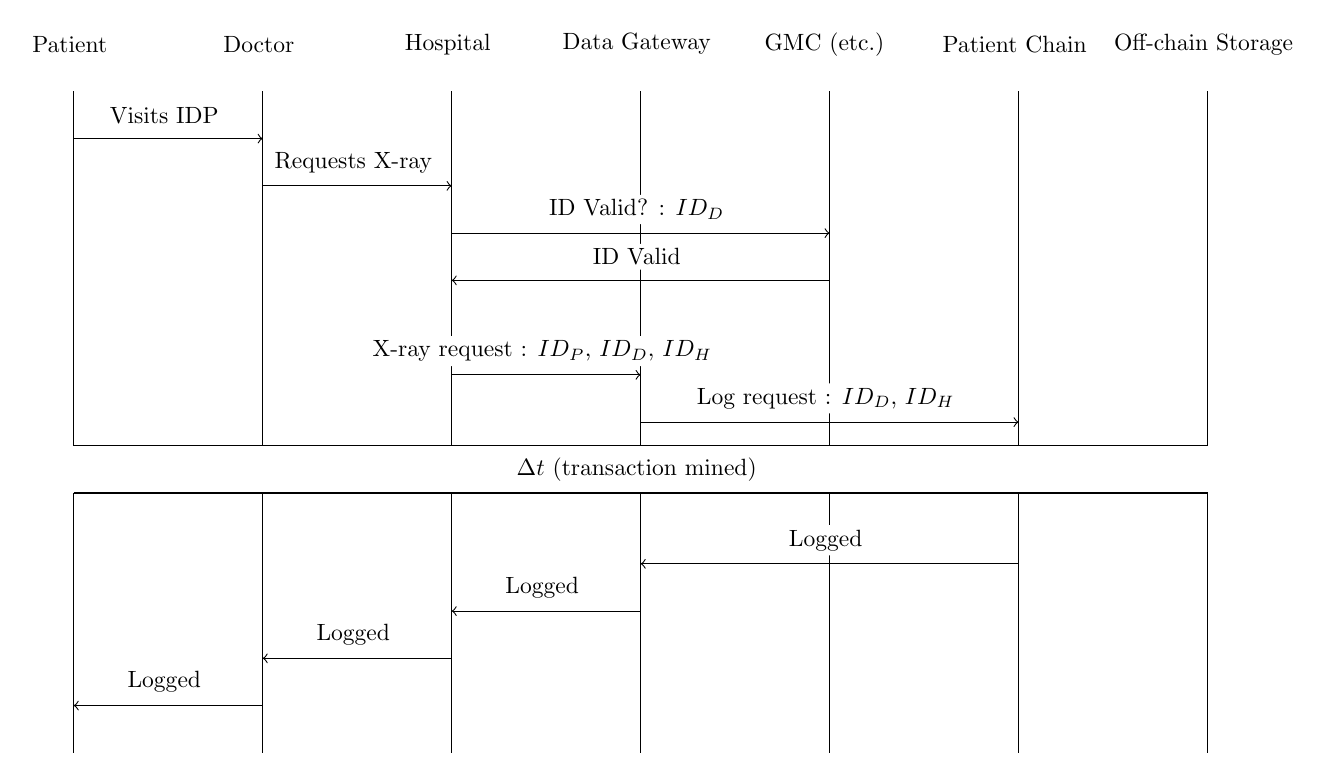
\begin{tikzpicture}[scale = 0.6, every node/.style={scale = 0.85}]

  % Lines
  \draw (4, 6) -- (4, 11.5);
  \draw (4, 12.5) -- (4, 20);
  \draw (8, 6) -- (8, 11.5);
  \draw (8, 12.5) -- (8, 20);
  \draw (12, 6) -- (12, 11.5);
  \draw (12, 12.5) -- (12, 20);
  \draw (16, 6) -- (16, 11.5);
  \draw (16, 12.5) -- (16, 20);
  \draw (20, 6) -- (20, 11.5);
  \draw (20, 12.5) -- (20, 20);
  \draw (24, 6) -- (24, 11.5);
  \draw (24, 12.5) -- (24, 20);
  \draw (28, 6) -- (28, 11.5);
  \draw (28, 12.5) -- (28, 20);

  % Headings
  \node[fill = white, rounded corners = 2pt, inner sep = 2pt, align = center] at (4, 21) { Patient };
  \node[fill = white, rounded corners = 2pt, inner sep = 2pt, align = center] at (8, 21) { Doctor };
  \node[fill = white, rounded corners = 2pt, inner sep = 2pt, align = center] at (12, 21) { Hospital };
  \node[fill = white, rounded corners = 2pt, inner sep = 2pt, align = center] at (16, 21) { Data Gateway };
  \node[fill = white, rounded corners = 2pt, inner sep = 2pt, align = center] at (20, 21) { GMC (etc.) };
  \node[fill = white, rounded corners = 2pt, inner sep = 2pt, align = center] at (24, 21) { Patient Chain };
  \node[fill = white, rounded corners = 2pt, inner sep = 2pt, align = center] at (28, 21) { Off-chain Storage };

  % Arrows
  \node[fill = white, rounded corners = 2pt, inner sep = 2pt, align = center] at (6, 19.5) { Visits IDP };
  \draw [ -> ] (4, 19) -- (8, 19);

  \node[fill = white, rounded corners = 2pt, inner sep = 2pt, align = center] at (10, 18.5) { Requests X-ray };
  \draw [ -> ] (8, 18) -- (12, 18);

  \node[fill = white, rounded corners = 2pt, inner sep = 2pt, align = center] at (16, 17.5) { ID Valid? : $ID_{D}$ };
  \draw [ -> ] (12, 17) -- (20, 17);

  \node[fill = white, rounded corners = 2pt, inner sep = 2pt, align = center] at (16, 16.5) { ID Valid \checkmark };
  \draw [ -> ] (20, 16) -- (12, 16);

  \node[fill = white, rounded corners = 2pt, inner sep = 2pt, align = center] at (14, 14.5) { X-ray request : $ID_{P}$, $ID_{D}$, $ID_{H}$ };
  \draw [ -> ] (12, 14) -- (16, 14);

  \node[fill = white, rounded corners = 2pt, inner sep = 2pt, align = center] at (20, 13.5) { Log request : $ID_{D}$, $ID_{H}$ };
  \draw [ -> ] (16, 13) -- (24, 13);

  \draw (4, 12.5) -- (28, 12.5);
  \node[fill = white, rounded corners = 2pt, inner sep = 2pt, align = center] at (16, 12) { $\Delta t$ (transaction mined) };
  \draw (4, 11.5) -- (28, 11.5);

  \node[fill = white, rounded corners = 2pt, inner sep = 2pt, align = center] at (20, 10.5) { Logged \checkmark };
  \draw [ -> ] (24, 10) -- (16, 10);

  \node[fill = white, rounded corners = 2pt, inner sep = 2pt, align = center] at (14, 9.5) { Logged \checkmark };
  \draw [ -> ] (16, 9) -- (12, 9);

  \node[fill = white, rounded corners = 2pt, inner sep = 2pt, align = center] at (10, 8.5) { Logged \checkmark };
  \draw [ -> ] (12, 8) -- (8, 8);

  \node[fill = white, rounded corners = 2pt, inner sep = 2pt, align = center] at (6, 7.5) { Logged \checkmark };
  \draw [ -> ] (8, 7) -- (4, 7);

  \end{tikzpicture}
  \caption{
    Doctor requests that patient have X-ray taken
  }
  \label{fig:user_story_01}
\end{figure}
